\documentclass[11pt]{article}
\usepackage{datetime}
\usepackage{color,array,graphics}
\usepackage{enumerate}
\usepackage[pdftex, colorlinks, linkcolor=red,citecolor=red,urlcolor=blue]{hyperref}
\usepackage{ulem}
\usepackage[vlined,ruled,commentsnumbered,linesnumbered]{algorithm2e}

\title{Visualize Profile}
\author{Ruochen Kong}
\date{}

\setlength{\parindent}{0cm}
\setlength{\parskip}{0.3cm plus4mm minus3mm}

\textwidth  6.5in
\oddsidemargin +0.0in
\evensidemargin +0.0in
\textheight 9.0in
\topmargin -0.5in
\linespread{1.4}

\usepackage{upquote,textcomp}
\usepackage{amssymb,amsmath,amsfonts,amsthm}
\usepackage{graphicx}
\usepackage{multicol}
\usepackage{float}
\usepackage{multirow}
\usepackage{stmaryrd}
\usepackage{mathrsfs} 
\usepackage{makecell, rotating}
\usepackage{pdfpages}

\newcommand{\vect}[1]{{\bf #1}}                 %for bold chars
\newcommand{\vecg}[1]{\mbox{\boldmath $ #1 $}}  %for bold greek chars
\newcommand{\matx}[1]{{\bf #1}}

\def\OR{\vee}
\def\AND{\wedge}
\def\imp{\rightarrow}
\def\math#1{$#1$}

\DeclareSymbolFont{AMSb}{U}{msb}{m}{n}
\DeclareMathSymbol{\N}{\mathbin}{AMSb}{"4E}
\DeclareMathSymbol{\Z}{\mathbin}{AMSb}{"5A}
\DeclareMathSymbol{\R}{\mathbin}{AMSb}{"52}
\DeclareMathSymbol{\Q}{\mathbin}{AMSb}{"51}
\DeclareMathSymbol{\I}{\mathbin}{AMSb}{"49}
\DeclareMathSymbol{\C}{\mathbin}{AMSb}{"43}

\usepackage{tikz}


\begin{document}
\maketitle{}
\section{Additional information}
\begin{enumerate}
	\item All the codes used in this lab is stored on \href{https://github.com/RuochenKong/BMI500Labs}{GitHub} under the \href{https://github.com/RuochenKong/BMI500Labs/tree/master/lab1}{\textit{lab1}} folder.
	\item The code used as peer review under the \href{https://github.com/RuochenKong/BMI500Labs/tree/master/lab1/prev_python_codes}{\textit{lab1/prev\_python\_codes}}. The code was written to assist a Chinese mobile game, so the name and its data are in Chinese. Hence, I did the code review with \textbf{Zheyuan Zhang}.
\end{enumerate}
\textit{I changed the repo from private to public to make the grading process easier.}

\section{Visualize and Analyze the Profile}

	\begin{figure}[h]
		\centering
		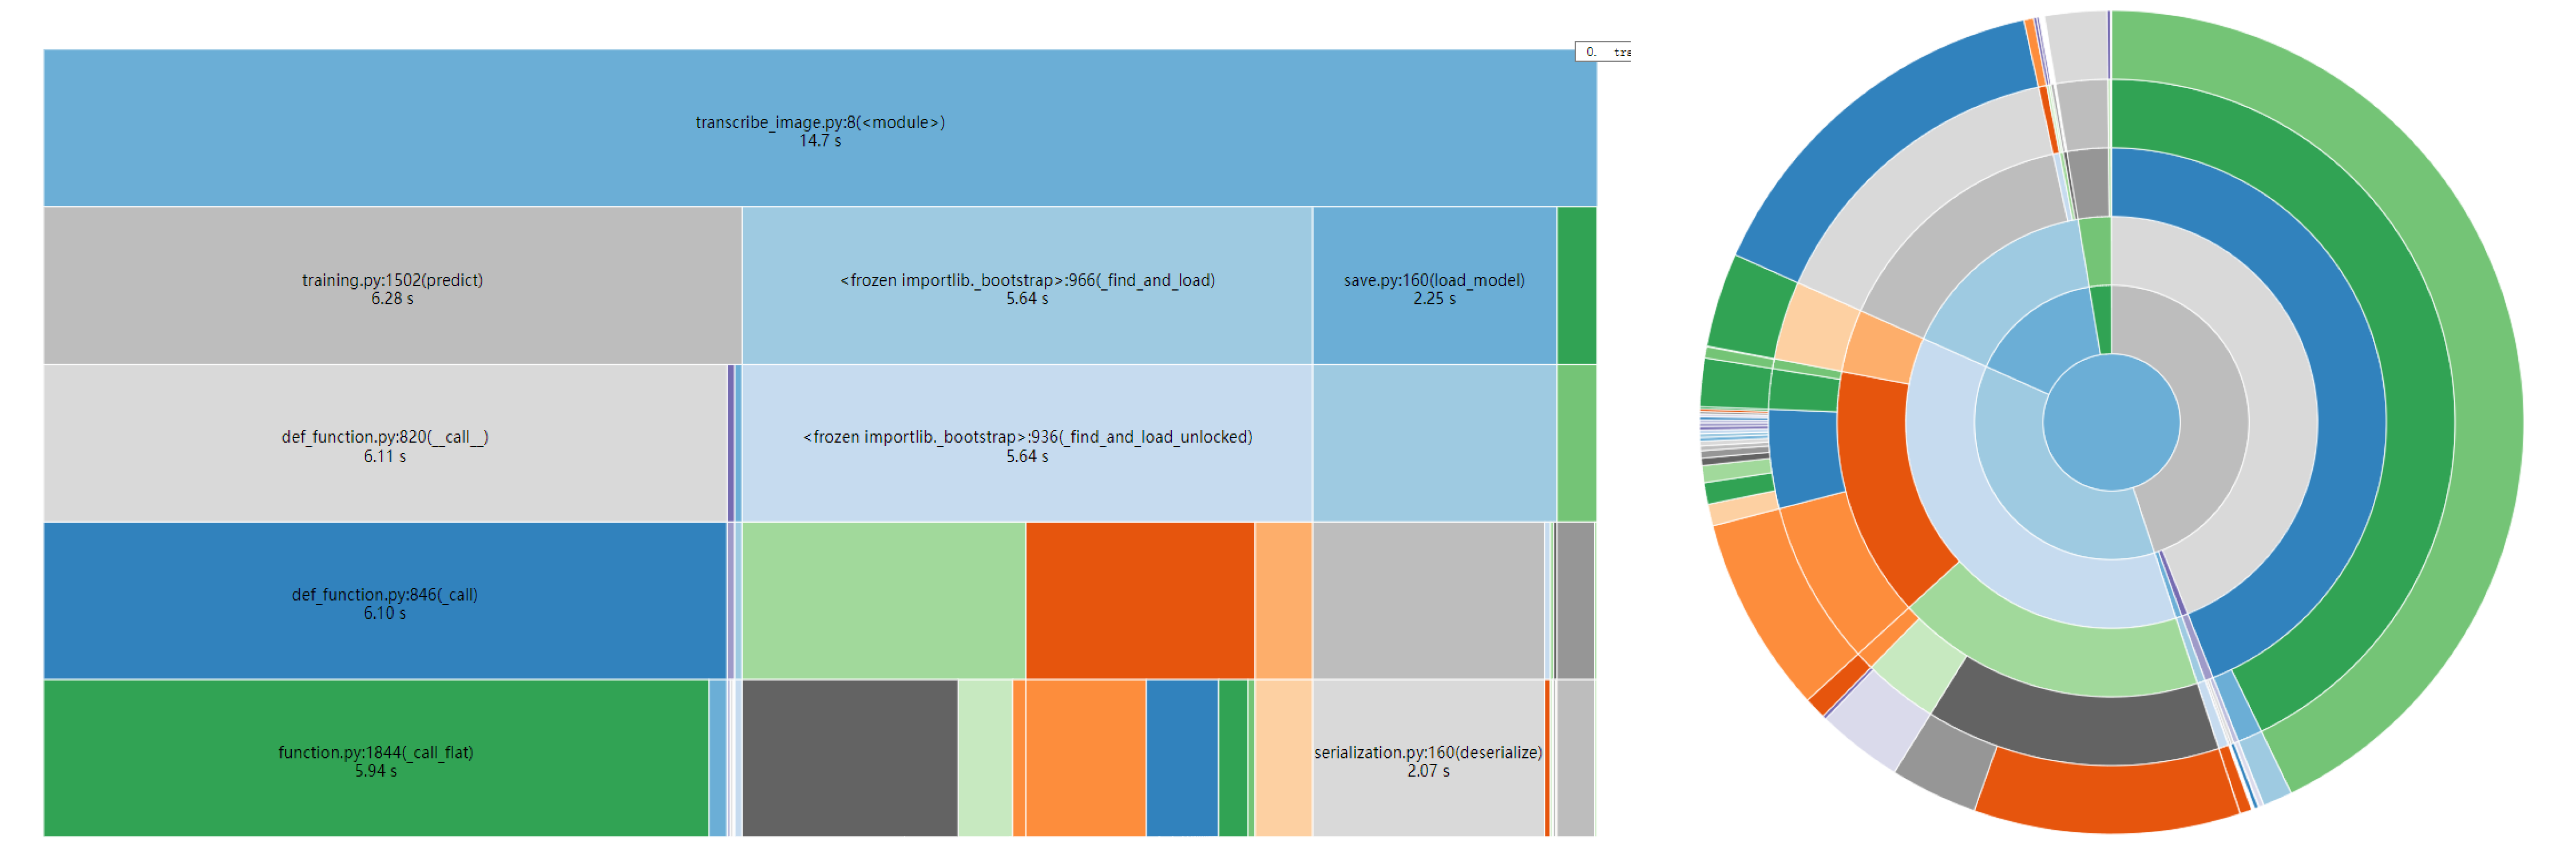
\includegraphics[width=0.9\textwidth]{prof_viz.png}
		\caption{Visualization of the profile with SnakeViz}
		\label{fig:viz}
	\end{figure}

	From the visualization, we can see that the running time on predicting and loading is similar. Specificly, 42.6\% of time was in predicting, while 38.3\% was in finding and loading. The remaning time mostly spent on load the csv file and the model, which is about 17.7\%. According to the values, the speed of this \textit{transcribe\_image.py} largely depends on the speed of loading files.\\

	\textbf{\textit{The following pages are the first 5 pages of the SnakeViz Result.}}

\newpage
\includepdf[pages=1-5]{KONG_ImageTrans_Profile_full.pdf}

\end{document}
